\documentclass[11pt,french,]{article}
\usepackage{lmodern}
\usepackage{amssymb,amsmath}
\usepackage{ifxetex,ifluatex}
\usepackage{fixltx2e} % provides \textsubscript
\ifnum 0\ifxetex 1\fi\ifluatex 1\fi=0 % if pdftex
  \usepackage[T1]{fontenc}
  \usepackage[utf8]{inputenc}
\else % if luatex or xelatex
  \ifxetex
    \usepackage{mathspec}
  \else
    \usepackage{fontspec}
  \fi
  \defaultfontfeatures{Ligatures=TeX,Scale=MatchLowercase}
\fi
% use upquote if available, for straight quotes in verbatim environments
\IfFileExists{upquote.sty}{\usepackage{upquote}}{}
% use microtype if available
\IfFileExists{microtype.sty}{%
\usepackage{microtype}
\UseMicrotypeSet[protrusion]{basicmath} % disable protrusion for tt fonts
}{}
\usepackage[margin=1in]{geometry}
\usepackage{hyperref}
\hypersetup{unicode=true,
            pdftitle={Rapport du Projet HMSN204},
            pdfauthor={Mathieu Blaison, Sean Laidlaw},
            pdfborder={0 0 0},
            breaklinks=true}
\urlstyle{same}  % don't use monospace font for urls
\ifnum 0\ifxetex 1\fi\ifluatex 1\fi=0 % if pdftex
  \usepackage[shorthands=off,main=french]{babel}
\else
  \usepackage{polyglossia}
  \setmainlanguage[]{french}
\fi
\usepackage{longtable,booktabs}
\usepackage{graphicx,grffile}
\makeatletter
\def\maxwidth{\ifdim\Gin@nat@width>\linewidth\linewidth\else\Gin@nat@width\fi}
\def\maxheight{\ifdim\Gin@nat@height>\textheight\textheight\else\Gin@nat@height\fi}
\makeatother
% Scale images if necessary, so that they will not overflow the page
% margins by default, and it is still possible to overwrite the defaults
% using explicit options in \includegraphics[width, height, ...]{}
\setkeys{Gin}{width=\maxwidth,height=\maxheight,keepaspectratio}
\IfFileExists{parskip.sty}{%
\usepackage{parskip}
}{% else
\setlength{\parindent}{0pt}
\setlength{\parskip}{6pt plus 2pt minus 1pt}
}
\setlength{\emergencystretch}{3em}  % prevent overfull lines
\providecommand{\tightlist}{%
  \setlength{\itemsep}{0pt}\setlength{\parskip}{0pt}}
\setcounter{secnumdepth}{0}
% Redefines (sub)paragraphs to behave more like sections
\ifx\paragraph\undefined\else
\let\oldparagraph\paragraph
\renewcommand{\paragraph}[1]{\oldparagraph{#1}\mbox{}}
\fi
\ifx\subparagraph\undefined\else
\let\oldsubparagraph\subparagraph
\renewcommand{\subparagraph}[1]{\oldsubparagraph{#1}\mbox{}}
\fi

%%% Use protect on footnotes to avoid problems with footnotes in titles
\let\rmarkdownfootnote\footnote%
\def\footnote{\protect\rmarkdownfootnote}

%%% Change title format to be more compact
\usepackage{titling}

% Create subtitle command for use in maketitle
\newcommand{\subtitle}[1]{
  \posttitle{
    \begin{center}\large#1\end{center}
    }
}

\setlength{\droptitle}{-2em}

  \title{Rapport du Projet HMSN204}
    \pretitle{\vspace{\droptitle}\centering\huge}
  \posttitle{\par}
    \author{\emph{Mathieu Blaison, Sean Laidlaw}}
    \preauthor{\centering\large\emph}
  \postauthor{\par}
    \date{}
    \predate{}\postdate{}
  
\usepackage{float}
\usepackage{longtable}
\usepackage{fancyhdr}
\usepackage{upgreek}
\usepackage{setspace}
\usepackage{pdfpages}
\pagestyle{fancy}
\fancyhead[LE,RO]{}
\fancyhead[LO,RE]{}
\renewcommand{\headrulewidth}{0.4pt}
\renewcommand{\footrulewidth}{0pt}
\fancyhead[LO,RE]{Blaison, Laidlaw}
\fancyhead[RO,LE]{Projet HMSN204}
\fancyfoot[L]{Université de Montpellier}
\fancyfoot[C]{\thepage}
\fancyfoot[R]{Master 1 SNS BCD}
\definecolor{sll_blue}{RGB}{10,99,181}
\hypersetup{colorlinks,citecolor=black,filecolor=black,linkcolor=sll_blue,urlcolor=sll_blue}

\begin{document}
\maketitle

\hypertarget{introduction}{%
\section{Introduction}\label{introduction}}

Au début du projet nous avons tout d'abord eu une phase de réfexion
initiale dsur le projet. Nous avons ainsi établi le diagramme de Gantt
suivant.

\begin{figure}[h]
 \centering
 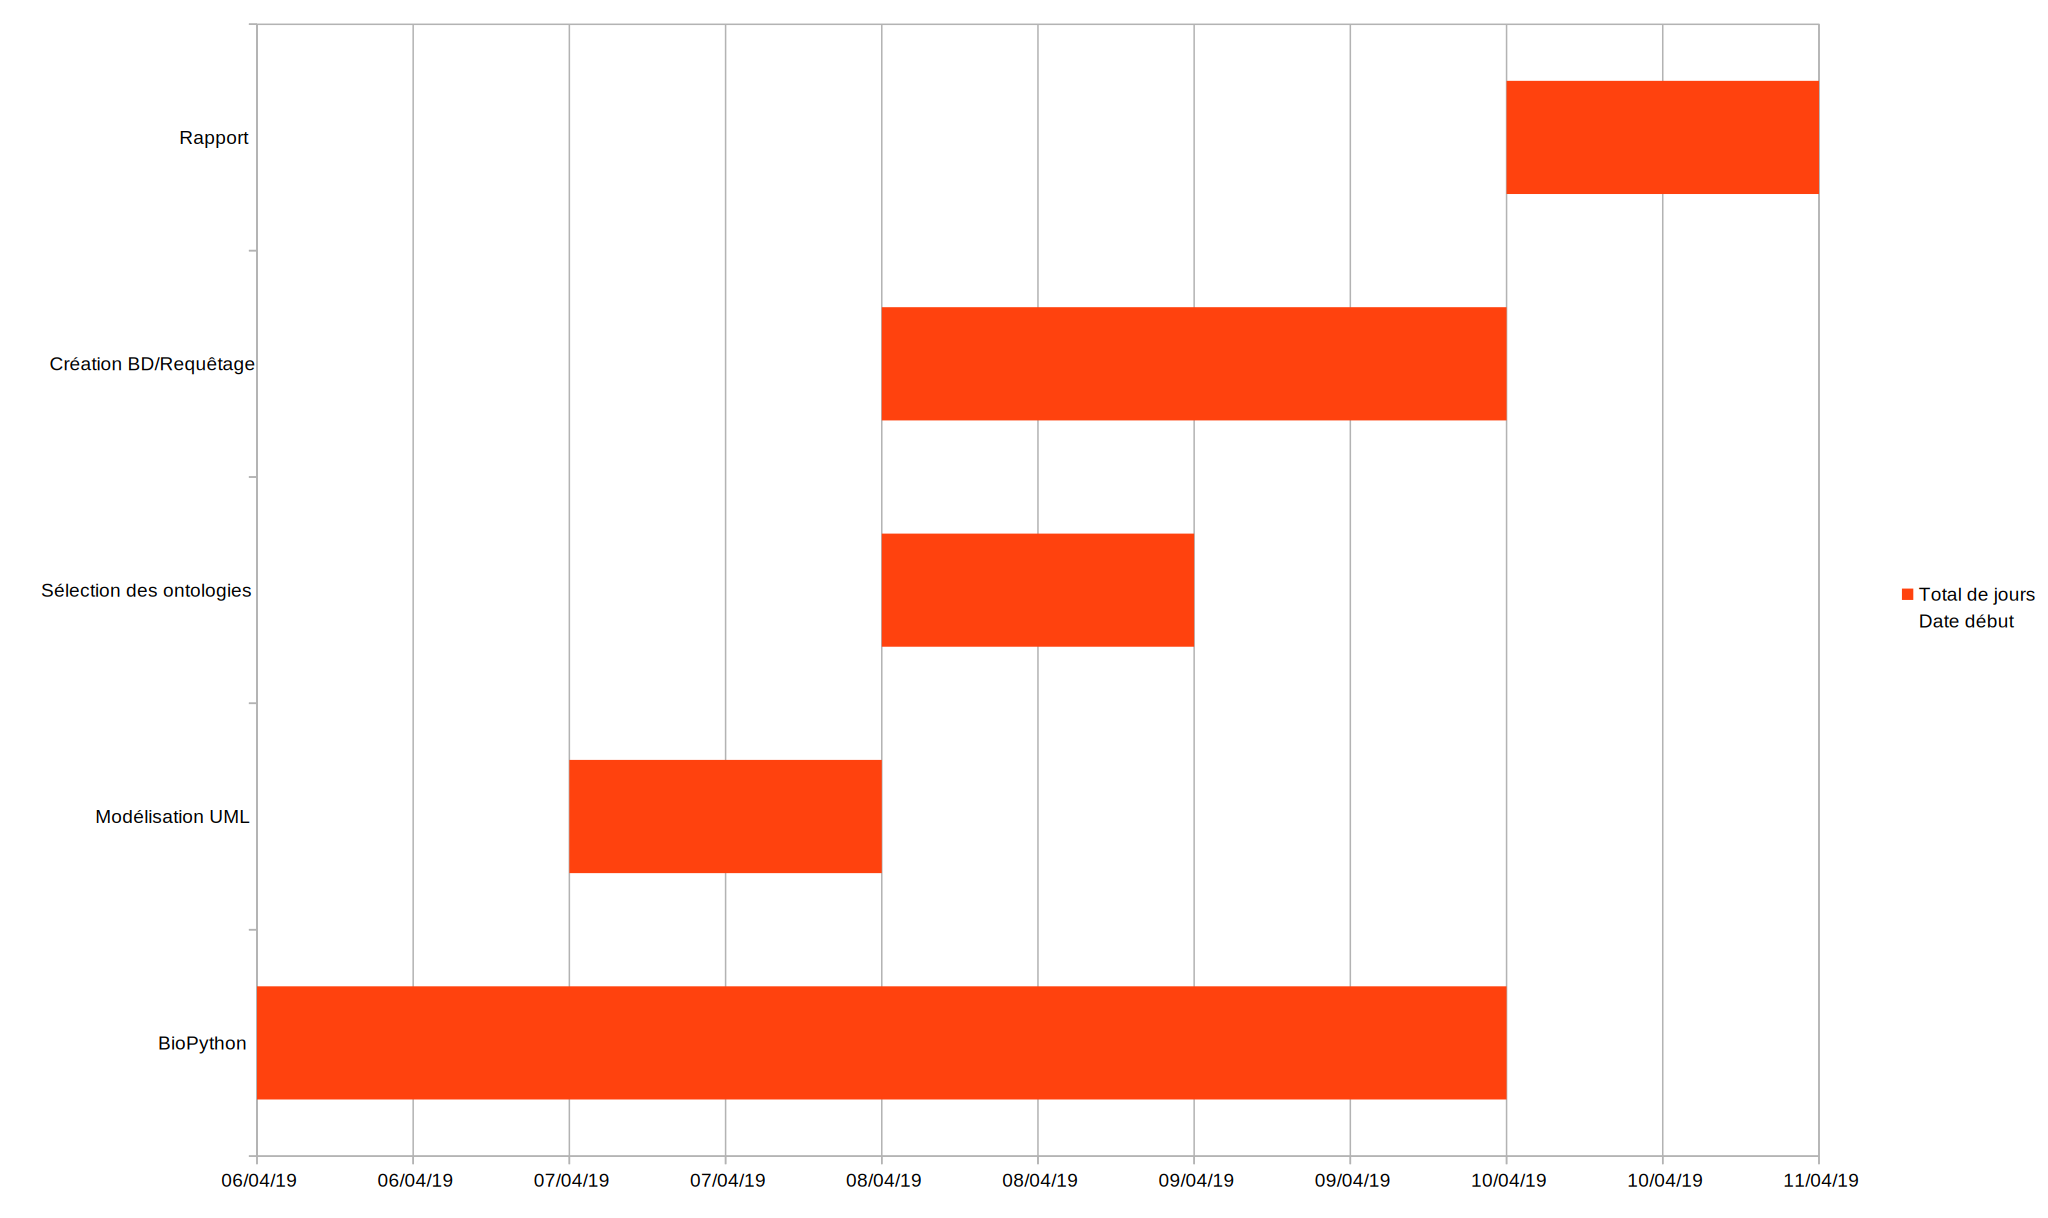
\includegraphics{../img/Gantt.pdf}
 \caption{Diagramme de Gantt détaillant le partage des responsabilités par rapport au temps}
\end{figure}

De cette réflexion initiale surle projet nous avons pu en établir le
diagramme de cas d'utilisation suivant.

\begin{figure}[H]
 \centering
 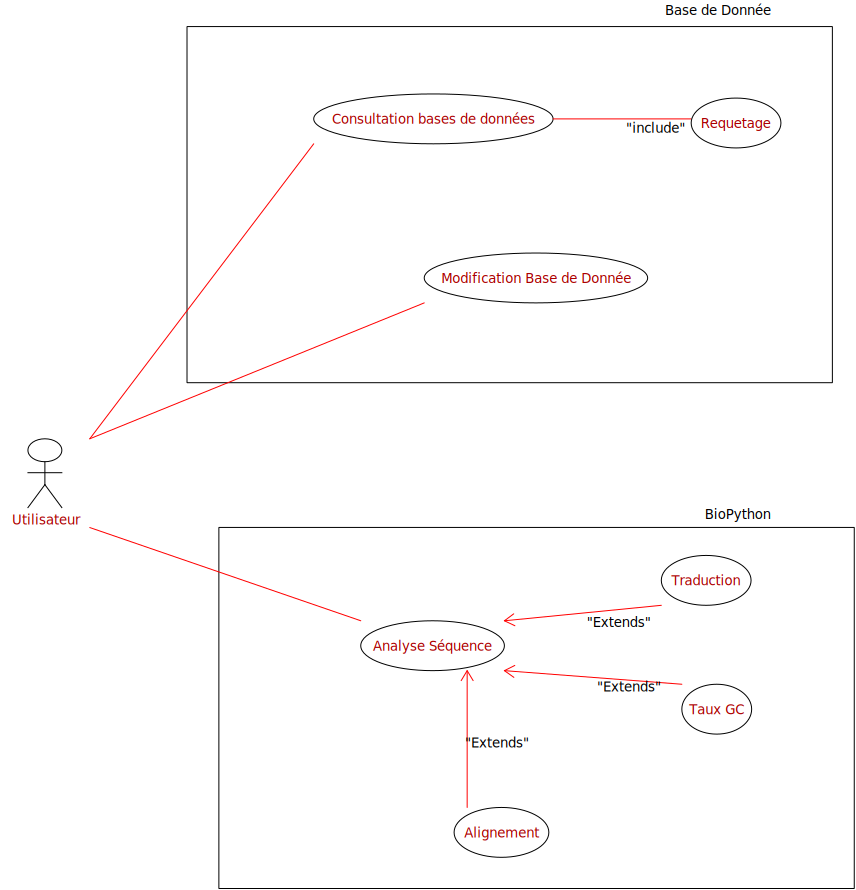
\includegraphics{../img/Cas_utilisation.pdf}
 \caption{Diagramme de Cas d'Utilisation}
\end{figure}

\hypertarget{traitements-biopythons-et-manipulation-des-sequences}{%
\section{Traitements Biopythons et manipulation des
séquences}\label{traitements-biopythons-et-manipulation-des-sequences}}

\hypertarget{obtention-des-sequences}{%
\subsection{Obtention des sequences}\label{obtention-des-sequences}}

Le jeu de données étant collectionné afin de mieux comprendre les
mécanismes physiologiques liés à la croissance des plantes, on a choisi
d'étudier le gène SEX1, qui a un rôle dans le dégradation de l'amidon.

Afin de pouvoir démontrer les résultats, le code utilisé, et les
explications, on a choisi d'utiliser un Jupyter Notebook. Dans ce
dernier nous avons écrit une fonction qui obtient le fichier fasta via
une requête Entrez correspondant à l'ARN messager.

Pour l'obtention des séquences mutés cependant, il y avait un choix à
faire. En effet, en recherchant la base de données NCBI avec la requête
\texttt{SEX1{[}Gene{]}\ AND\ Arabidopsis\ thaliana{[}Organism{]}}, on
constate qu'il y a 3 ARNm différents répondant à ces critères. En
regardant de plus près cependant, on voit que ce sont des variants
d'épissage. Alors que le plupart des aligneurs modernes sont
\emph{splice-aware}, l'aligneur que nous avons construit effectue un
alignement globale à la base de l'algorithme Needleman-Wunsch et donc ne
l'est pas. Ceci veut dire qu'on ne pourrait pas correctement aligner les
variants d'épissage contre notre séquence sauvage. Afin d'obtenir une
séquence contre lequel on pourrait aligner notre fasta sauvage, on a
consulté la base de donnée dbSNP qui détail le
\href{https://www.ncbi.nlm.nih.gov/SNP/snp_ref.cgi?locusId=837619}{liste
des SNP de la gène SEX1}, leurs localisations dans l'ARN messager, et
les identifiants de ces SNP. Un peu de vimscript plus tard, et 1/4 des
SNP détaillés sur dbSNP étaient appliqués à la fasta du SEX1 sauvage. Le
fasta mutant produit, a ensuite été ajouté au projet GitHub afin que le
notebook Jupyter puisse le telecharger pour le transformer en objet Seq
et l'aligner contre la séquence sauvage.

\begin{longtable}[]{@{}llll@{}}
\caption{Liste des identifiants dbSNP utilisés pour creer le fasta
mutant}\tabularnewline
\toprule
Used dbSNP IDs & & &\tabularnewline
\midrule
\endfirsthead
\toprule
Used dbSNP IDs & & &\tabularnewline
\midrule
\endhead
rs1105066589 & rs1103971843 & rs1095089377 & rs1100808719\tabularnewline
rs1095780989 & rs1095659046 & rs1097407346 & rs1097236347\tabularnewline
rs1105152302 & rs1097124183 & rs347038182 & rs346885812\tabularnewline
rs1101762250 & rs1100942745 & rs1106840358 & rs346897346\tabularnewline
rs1099291378 & rs1102995172 & rs1096948278 & rs1099609436\tabularnewline
rs1104510198 & & &\tabularnewline
\bottomrule
\end{longtable}

\hypertarget{alignement-globale}{%
\subsection{Alignement Globale}\label{alignement-globale}}

Afin d'aligner les deux séquences, on a utilisé les dataframe de la
librarie Pandas. Étant l'objet qui s'approchait le plus d'un tableau, et
permettant l'écriture d'une de ses cases avec seulement les coordonnés
de la case, il a paru d'être la meilleur solution.

Le déroulement de l'alignement se passe dans plusieurs étapes. D'abord
il y a l'initiation du tableau, ou le script parcours la longueur des
deux séquences convertant chaque nucléotide d'une en colonne et chaque
nucléotide de l'autre en ligne.

\newpage

Ensuite, pour la remplissage du tableau les cases ont été remplis avec
les valeurs correspondant au statut de match ou mismatch de la
nucléotide, ainsi que le score de ses cases voisins d'en haut, à gauche,
et en diagonale. En plus de déposant le score dans la case du premier
dataframe, une symbole représentant la direction à été inséré dans un
autre tableau (\textless, , ou \textbar{} ) afin que la fonction
suivante puisse suivre le chemin parcouru.

Une fois le tableau rempli, le chemin de retour a été tracé par la
fonction traceback qui exploite le modèle de double tableau afin de se
baser à la fois sur le score le plus haut, et puis de se déplacer dans
la direction qui à amené à ce score. Ensuite avec un alignement obtenu
les positions de variations sauvage/mutés, le taux de GC, et la
traduction en séquence dacides aminés sont données.

\begin{figure}[H]
 \centering
 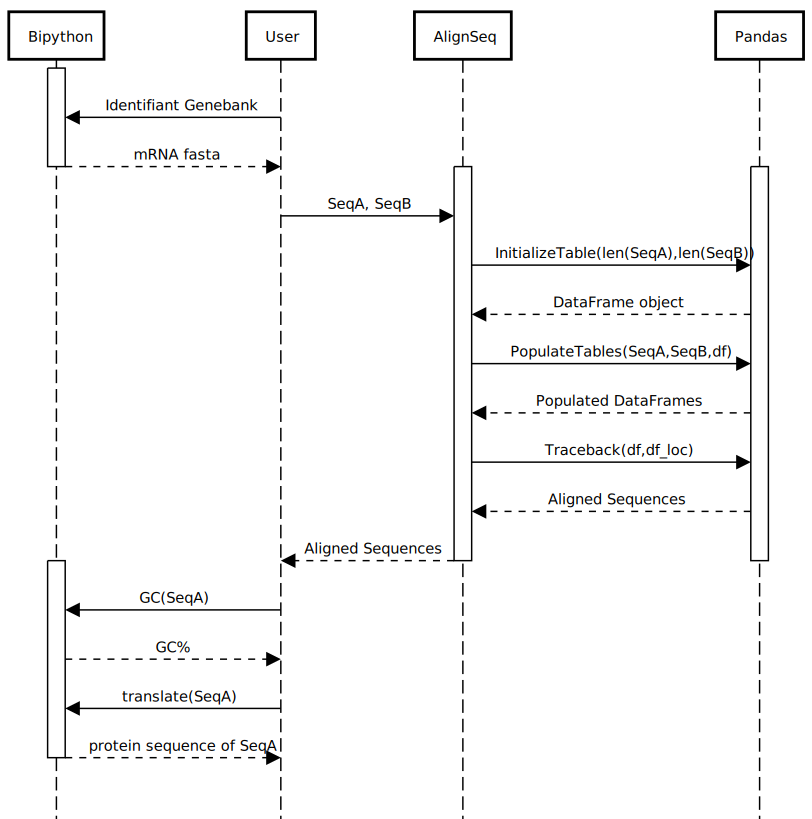
\includegraphics{../img/AlignmentGlobale.pdf}
 \caption{Diagramme de séquence pour alignement globale}
\end{figure}

\hypertarget{optimisations}{%
\subsubsection{Optimisations}\label{optimisations}}

L'algorithme utilisé pour l'alignement globale souffre de la problème de
complexité. En effet, la génération et la remplissage du tableau
augmente quadratiquement avec les longeurs de sequences fournis. Où m
est le longeur de seqX et n le longueur de seqY, la complexité de temps
d'une alignement par cette méthode serait de l'ordre de O(m*n). Pour les
séquences recherchés dans ce projet, les longueurs de séquence était à
l'ordre du millier, rendant l'alignement très lent.

Afin d'essayer de contourner le problème, des optimisations ont été
recherchés. Python n'étant pas la plus vite des langages, nous a amener
à utiliser la librairie cython qui convertiras certains de nos fonctions
en code C afin de profiter d'une meilleure performance. De plus, on a
essayé également de mettre certains fonctions en cache, pour pas qu'il
soit recalculé à chaque fois, et enfin on a essayé la librairie JIT qui
fait une compilation à la volée. Ce dernier a donnée les résultats les
plus prometteurs, mais n'as pas fonctionné avec la fonction le plus
lourd de l'alignement car il n'est pas compatible avec pandas.

\begin{longtable}[]{@{}ll@{}}
\caption{Comparaisons d'optimisations et performances}\tabularnewline
\toprule
Optimisation & Alignment Time (s)\tabularnewline
\midrule
\endfirsthead
\toprule
Optimisation & Alignment Time (s)\tabularnewline
\midrule
\endhead
None & 18.6\tabularnewline
Function Caching & 18.16\tabularnewline
Cython & 18.02\tabularnewline
JIT Compilation & 18.22\tabularnewline
Combined & 18.55\tabularnewline
\bottomrule
\end{longtable}

\hypertarget{base-de-donnees}{%
\section{Base de données}\label{base-de-donnees}}

\hypertarget{reflexion-sur-la-base-de-donnees}{%
\subsection{Réflexion sur la base de
données}\label{reflexion-sur-la-base-de-donnees}}

On a eu le choix d'un des SGBD vu ce semestre : chado/postgresql (module
phenotype), relationnel seul (oracle, postgresqlou mysql), neo4j,
couchdb, triplestore jena/rdf.

Notre choix s'est ainsi porté sur la base de données Chado. Celle-ci est
conçue spécialement pour gérer les représentations complexes de données
biologiques. Chado va également posséder des modules permettant de gérer
spécifiquement les relations entre termes ontologiques. Pour créer sa
base de données Chado utilise le système de gestion PostgreSQL. Ayant
deja des bases en SQL , ce choix nous a ainsi paru judicieux pour
pouvoir réaliser une implémentation correcte de la base de données avec
un temps limité et la taille de notre groupe.

\hypertarget{modelisation-de-la-base-de-donnees}{%
\subsection{Modélisation de la base de
données}\label{modelisation-de-la-base-de-donnees}}

Avant de nous lancer dans la création de notre base de donnée il faut
d'abord la penser. Pour ce faire le meilleur moyen est de se représenter
la base de données visuellement à l'aide d'un shéma UML et plus
particulièrement d'un diagramme de classes. Notre bases de données se
divise en ``deux'' parties. Une gérant les données issues des
expérimentations des M1 BFP et l'autre gérant les termes d'ontologies.
Un lien est fait entre ces 2 parties au niveau de la table phénotype.
Avec le recul cette manière de faire n'était probablement pas la
meilleure et des améliorations doivent être apportés principalement pour
la partie gérant l'ontologie.

Nous retrouvons ansi avec une base de données corrspondant au diagramme
de classe suivant:

\begin{figure}[h]
 \centering
 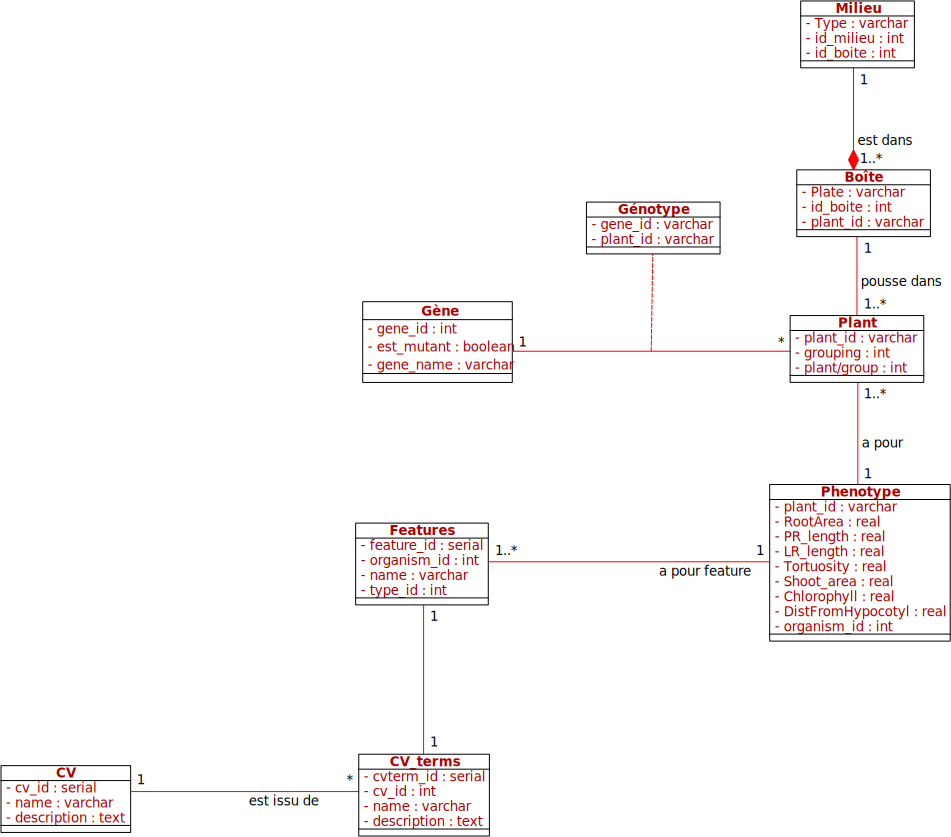
\includegraphics{../img/class_diagram.pdf}
 \caption{Diagramme de classe}
\end{figure}

\hypertarget{ontologie}{%
\subsection{Ontologie}\label{ontologie}}

Il a ainsi fallu penser à la manière d'intégrer l'ontologie dans notre
base de données . L'ontologie va représenter des concepts (comme une
caractéristique phénotypique) et les relations que ces concepts peuvent
partager. Dans notre cas on s'est intéressé à rechercher les relations
entre les termes ontologiques constituant les phénotypes observés et
mesurés par les étudiants BFP. Pour ce faire ces phénotypes ont été
``décomposé'' en plusieurs et leur terme ontologique ont été associé en
une relation. Par exemple, la longueur de la racine primaire va
corrrespondre à une longueur de racine (possédant son terme ontologique)
qui ferait partie (is part of) d'une racine primaire(possédant aussi son
propre terme ontologique). ces données générées seront ensuite insérées
dans notre base de données. Ces données peuvent être récupérées grâce à
de nombreuses ressources regroupant les termes d'ontologies appartenant
à un même ``groupe''.

\hypertarget{implementation-bases-de-donnees-et-peuplement}{%
\subsection{Implémentation bases de données et
peuplement}\label{implementation-bases-de-donnees-et-peuplement}}

\hypertarget{creation-des-tables}{%
\subsubsection{Création des tables}\label{creation-des-tables}}

Afin de créer les tables un script SQL de création de ces tables à été
écrit. Celui-ci va constituer dans un premier temps en la destruction
des tables et de leurs contraintes dans le cas à l'aide d'un drop table.
Il va ensuite permettre de construire ces tables en affectant les clefs
primaires et étrangères appropriés à chaque table.

Afin de générer les tables nécessaires à l'ontologie, le module cv de
Chado à été utilisé. Je me rends compte cependant à l'écriture de ce
rapport que j'ai mal compris et mal utilisé ce module cv, notamment en
n'utilisant pas la table cv\_term relationship.

\hypertarget{insertion-des-donnees-dans-les-tuples}{%
\subsubsection{Insertion des données dans les
tuples}\label{insertion-des-donnees-dans-les-tuples}}

Afin de ne pas avoir à insérer les données issues du document csv qui
nous a été fourni manuellement dans nos tuples une réorganisation de
celles-ci a été effectué. Celle-ci ont ainsi été redistribuées sur
plusieurs fichier csv correspondant chacun à une table donnée. On peut
ensuite insérer les données contenues dans ces fichier dans nos tuples à
l'aide de la commande \texttt{\textbackslash{}\textbackslash{}copy} .
Les données ayant rapport à l'ontologie ont été insérées
``manuellement'' à l'aide de `insert values into'.

\hypertarget{requetes}{%
\subsection{Requêtes}\label{requetes}}

Des requêtes ont été généré afin d'interroger notre base de données. Ces
reqûetes ont été regroupées dans un script . Ces requêtes m'ont permis
de me rendre compte que certains éléments de la base de donnée auraient
mérités à être pensé autrement afin de pouvoir faire des requêtes plus
précise et intéressantes au niveau de l'ontologie.

Exemple de requête effectué:

Observe le potentiel effet du milieu sur la taille moyenne de l'aire
racinaire

\begin{verbatim}
select m.type, avg(ph.Root_area)
from milieu m, boite b, plant p, phenotype ph
where m.id_boite = b.id_boite and b.plant_id = p.plant_id and p.plant_id = ph.plant_id
group by m.type;
\end{verbatim}

\begin{longtable}[]{@{}ll@{}}
\caption{Résultat de la requête}\tabularnewline
\toprule
gene\_name & count\tabularnewline
\midrule
\endfirsthead
\toprule
gene\_name & count\tabularnewline
\midrule
\endhead
Col\_0 & 29\tabularnewline
nrt & 76\tabularnewline
sex1 & 11\tabularnewline
pgm & 11\tabularnewline
\bottomrule
\end{longtable}

\hypertarget{conclusion}{%
\section{Conclusion:}\label{conclusion}}

Ainsi nous avons été en mesure de générer une base de donnée permettant
de faire des requêtes pour la consultation et potentiellement
l'interprétation des résultats obtenus par les M1 BFP . Cette base de
données permet aussi de consulter les relations d'ontologies des
phénotypes mesurés. Cependant cette ontologie n'a pas été implémenté de
manière optimale par manque de comprhéension et de temps pour rattraper
les erreurs. Les séquences nucléiques des gènes o,t pu être récupéreés
depuis le NCBI puis elles ont pu être analysées àl'aide de BioPython
pour nous fournir des informations qui auraient pu être utilisées dans
notre base de données.


\end{document}
